\documentclass[sigconf]{acmart}

\usepackage{graphicx}
\usepackage{hyperref}
\usepackage{todonotes}

\usepackage{endfloat}
\renewcommand{\efloatseparator}{\mbox{}} % no new page between figures

\usepackage{booktabs} % For formal tables

\settopmatter{printacmref=false} % Removes citation information below abstract
\renewcommand\footnotetextcopyrightpermission[1]{} % removes footnote with conference information in first column
\pagestyle{plain} % removes running headers

\newcommand{\TODO}[1]{\todo[inline]{#1}}

\begin{document}
\title{Predicting Profitable Customers in Banking Industry}


\author{Dhanya Mathew}
\orcid{HID328}
\affiliation{%
  \institution{Indiana University}
  \streetaddress{711 N Park Ave}
  \city{Bloomington} 
  \state{Indiana} 
  \postcode{47408}
}
\email{dhmathew@iu.edu}


% The default list of authors is too long for headers}
\renewcommand{\shortauthors}{G. v. Laszewski}


\begin{abstract}
Banks often want to know the profile of their profitable top 1\% or 20\% customers looks like. Conversely they may also wonder what the general profile is of the customers in the worst 1\% and 20\% of profit. Based on customer’s data variables at any given time, a good predictive model can predict which profit group (extremely unprofitable, average, extremely profitable, etc.) customers falls into. This helps financial institutions to better understand what drives the customer profit and accordingly take decisions to sell their products to the right customers. Further down in banking sector, it is a challenge to identify customers who are most likely to repay a loan. Recent big data and machine learning technologies have the potential to predict good customers and open doors for banks to profitable growth. Since the banking sector has evolved over the periods, there are tremendous amount of historical data available to analyze. We show how bank's big data can be analyzed and create a model based on that, to classify customers. In addition to big data technologies, we used machine learning algorithms to build the predictive model to predict creditworthy and uncreditworthy customers from a list of new customers. Random forest classification algorithm is used to achieve this goal.

\end{abstract}

\keywords{i523, HID328, Big Data, Spark, Python, Decision Trees , Random Forest}


\maketitle



\section{Introduction}

Big data as the name implies, refers to large and complex data which continues to grow enormously day by day. Industries like financial firms, in particular, have widely adopted big data analytics to obtain better investment decisions with consistent growth. Recent survey research indicates that 71 percent of firms in the financial services industry at a global level are exploring big data and predictive analytics \cite{accenture-next-generation-financial}. This number continues to grow and sectors like government, business, technology, universities, health-care, finance, manufacturing etc make use of big data to obtain meaningful information using big data technologies \cite{wiki-bigdata}. 

The finance sector contributes to the daily data generation from products and marketing, banking, business, share market etc. Banking is a very sensitive field and any useful insight can make a positive impact on the overall turnover. Historic data analysis and real time data analysis are equally important in terms of banking sector. The era of big data helps financial firms to take quality business decisions related to expanding revenues, managing costs, hiring resources etc, based on effective data analysis which provide access to real-time insights. Data-driven decision making is one of the key advantages of big data technologies.

\subsection{Project Goals}

This project aims to help banking sector to identify profitable customers. Specifically, help banks to take a decision whether to approve or reject a loan application. When a new customer approaches the bank for a loan, banks would be able to identify the customers who are most likely to repay the loan by analyzing the applicant's profile and background information. 

There can be two scenarios of risks associated with the bank's decision. First, if the customer is creditworthy and if the bank rejects the loan, then it is a loss to the bank in terms of interest. Second, if the customer is uncreditworthy and if the bank approves the loan, then it is a loss to the bank in terms of loan amount and interest. Approving loan for an uncreditworthy customer will end up in more financial loss for the bank and accordingly is a greater risk. Hence banks would require a decision rule to follow for whom to approve the loan. With our model we are trying to mitigate these risks for the banks and contribute to the decision rules. In other words, our model helps to minimize the risks and maximize the profit.

\subsection{Methods and Technologies Involved}

We took a sample data set of loan applications from customers to a bank. In the real scenarios, we will not be able to apply analytical methods directly on the data as it likely be imperfect and containing irrelevant information. Hence we do data cleaning as the first step. Here we did data cleaning using spark. The cleaned data has 1000 customer records with 20 variables.

We did exploratory analysis like Chi-square test to understand data and for feature selection for analysis. We also did some graphical representations to show how the actual data is related and what are direct insights available from the cleaned data set.

To develop the model we first split the data set into two parts- training data and test data. We defined 2 baseline models, Trees and finally developed the Random Forest model. We compare all these models to identify the most effective and least penalty model. We did visualization and modelling using python.

\section{Data Set}

We used the German Credit data which is publically available in the UCI Machine Learning Repository \cite{uci} and also in the website of PennState Eberly College of Science \cite{psu-site}. Both these sites have the cleaned dataset and not the original one. Hence we recreated the original one from these data sets to understand and try out the data cleaning processes. Data sets include 1000 customer records and 20 variables and a class variable. In the class variable the actual class of the customer is specified - good or bad. The original data set in excel format is available in the github repository \cite{github}. Figure \ref{fig:Figure1} shows the first 10 rows of the original data set.

\begin{figure}[htb]
  \centering
  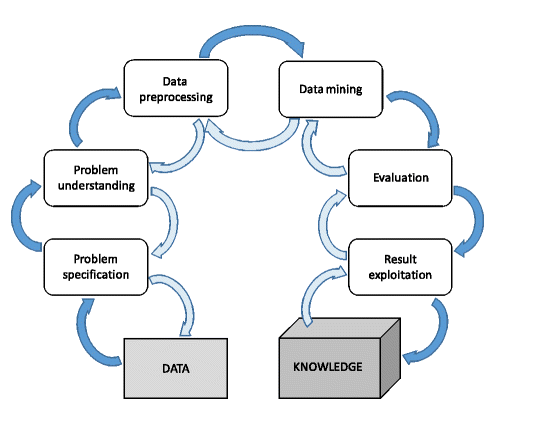
\includegraphics[width=1.0\columnwidth]{project/images/Figure1.png}
  \caption{First 10 rows of original data set
  \cite{github}}
  \label{fig:Figure1} 
\end{figure}

\begin{figure}[htb]
  \centering
  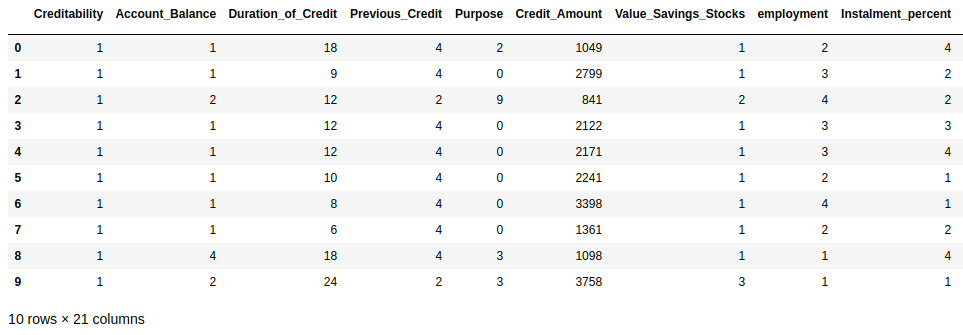
\includegraphics[width=1.0\columnwidth]{project/images/Figure2.png}
  \caption{First 10 rows of cleaned data set
  \cite{psu-site}}
  \label{fig:Figure2} 
\end{figure}

The cleaned data set we used in this project is taken from the website of PennState Eberly College of Science \cite{psu-site}. Figure \ref{fig:Figure2} shows first 10 rows from the cleaned data set. 

\section{Data Cleansing}



\section{Data Analysis}

\subsection{Exploratory Analysis}

Interquartile Range:

The interquartile range (IQR) is a measure of variability, based on dividing a data set into quartiles.

Quartiles divide a rank-ordered data set into four equal parts. The values that divide each part are called the first, second, and third quartiles; and they are denoted by Q1, Q2, and Q3, respectively.

Q1 is the "middle" value in the first half of the rank-ordered data set.
Q2 is the median value in the set.
Q3 is the "middle" value in the second half of the rank-ordered data set.
The interquartile range is equal to Q3 minus Q1.\cite{stat-trek-statistics}

Quartile:

Quartiles divide a rank-ordered data set into four equal parts. The values that divide each part are called the first, second, and third quartiles; and they are denoted by Q1, Q2, and Q3, respectively.

Note the relationship between quartiles and percentiles. Q1 corresponds to P25, Q2 corresponds to P50, Q3 corresponds to P75. Q2 is the median value in the set.

See also:  	AP Statistics Tutorial: Measures of Position



\subsection{Cross-Tabulation}

\section{Data Modelling}

\section{Results}



\section{Conclusion}

Put here an conclusion. Conlcusions and abstracts must not have any
citations in the section.


\begin{acks}

  The authors would like to thank Dr. Gregor von Laszewski for his
  support and suggestions to write this paper.

\end{acks}

\bibliographystyle{ACM-Reference-Format}
\bibliography{report} 


\end{document}
